\documentclass[tikz, border=2pt]{standalone}
\usepackage[none]{hyphenat}
\usepackage{helvet}
\renewcommand{\familydefault}{phv}

\begin{document}
\pagestyle{empty}

\definecolor{ltyellow}{rgb}{1.0, 1.0, 0.45} % 255/255/115
\definecolor{yellow}{rgb}{0.9, 0.9, 0.0} % % 230/230/0

\definecolor{ltorange}{rgb}{1.0, 0.74, 0.41} % 255/188/105
\definecolor{orange}{rgb}{0.96, 0.50, 0.0} % 246/127/0

\definecolor{ltred}{rgb}{1.0, 0.25, 0.25} % 255/64/64
\definecolor{red}{rgb}{0.79, 0.00, 0.01} % 201/0/3

\definecolor{ltpurple}{rgb}{0.81, 0.57, 1.00} % 206/145/255
\definecolor{purple}{rgb}{0.38, 0.00, 0.68} % 97/1/175

\definecolor{ltblue}{rgb}{0.67, 0.85, 0.91} % 171/217/233
\definecolor{blue}{rgb}{0.17, 0.48, 0.71} % 44/123/182

\definecolor{ltltgreen}{rgb}{0.7, 1.00, 0.7} % 96/204/14
\definecolor{ltgreen}{rgb}{0.37, 0.80, 0.05} % 96/204/14
\definecolor{green}{rgb}{0.23, 0.49, 0.03} % 59/125/8
  
\definecolor{dkslate}{rgb}{0.18, 0.21, 0.28} % 47/53/72
\definecolor{mdslate}{rgb}{0.45, 0.50, 0.68} % 114/127/173
\definecolor{ltslate}{rgb}{0.85, 0.88, 0.95} % 216/225/229

\definecolor{dkgray}{rgb}{0.25, 0.25, 0.25}
\definecolor{mdgray}{rgb}{0.50, 0.50, 0.50}
\definecolor{ltgray}{rgb}{0.75, 0.75, 0.75}


% From http://communities.usgs.gov/blogs/vis/typography-and-color/additional-colors/

% Main Colors
\definecolor{usgs_green}{HTML}{006F41}
\definecolor{usgs_teal}{HTML}{0061A3}
\definecolor{usgs_blue}{HTML}{0071B7}
\definecolor{usgs_navy}{HTML}{180F9B}
\definecolor{usgs_purple}{HTML}{8F009A}
\definecolor{usgs_red}{HTML}{FB0032}
\definecolor{usgs_orange}{HTML}{F99B00}

% USGS Dark Colors
\definecolor{usgs_dkgreen}{HTML}{1E4D2B}
\definecolor{usgs_dkgreen2}{HTML}{00443F}
\definecolor{usgs_dkblue}{HTML}{002F57}
\definecolor{usgs_dknavy}{HTML}{201258}
\definecolor{usgs_dkpurple}{HTML}{641B56}
\definecolor{usgs_dkred}{HTML}{881535}
\definecolor{usgs_dkorange}{HTML}{8D4200}


% USGS Light and Neutral Colors
\definecolor{usgs_ltblue}{HTML}{6AC3F2}
\definecolor{usgs_yellow}{HTML}{FFBD00}
\definecolor{usgs_ltgreen}{HTML}{66A48B}
\definecolor{usgs_ltgray}{HTML}{91B0BD}



\usetikzlibrary{positioning,arrows,shapes,calc,shadows.blur}

\tikzstyle{diagram} = [node distance=2.5em]

\tikzstyle{default} = [rectangle,
  %minimum text width=10em,
  minimum height=2.0em,
  text centered,
  line width=0pt,
  blur shadow={shadow blur steps=4},
]

\tikzstyle{root} = [
default,
font={\bfseries},
  top color=ltred!50!white,
  bottom color=ltred,
  anchor=west]

\tikzstyle{group} = [
  default,
  rounded corners=0.5em,
  top color=ltorange!50!white,
  bottom color=ltorange,
  anchor=west]

\tikzstyle{dataset} = [
  default,
  top color=ltblue!50!white,
  bottom color=ltblue,
  anchor=west]
  
\tikzstyle{xml} = [
  top color=ltgreen!50!white,
  bottom color=ltgreen,
  ]

\tikzstyle{legend} = [
  anchor=center]

\tikzstyle{subset-right} = [
  xshift=2em]

\newcommand{\variable}[1]{{\itshape #1}}
%\newcommand{\duscore}{\rule{8pt}{0.4pt}}
\newcommand{\duscore}{\_\_}

\tikzstyle{arrowto} = [line width=2pt, draw=white]



\begin{tikzpicture}[diagram]

  \node (workspace) [root] {Root (Workspace)};

  % Provenance
  \node (provenance) [below=of workspace.center, group, subset-right] {Provenance};
  \node (prov0) [below=of provenance.center, dataset, xml, subset-right] {\variable{SEIS-PROV XML}};
  \node (prov1) [below=of prov0.west, dataset, xml] {\variable{SEIS-PROV XML}};
  \node (prov2) [below=of prov1.west, dataset, xml] {\variable{SEIS-PROV XML}};
  \draw[arrowto] (workspace.south) |- (provenance.west);
  \draw[arrowto] (provenance.south) |- (prov0.west);
  \draw[arrowto] (provenance.south) |- (prov1.west);
  \draw[arrowto] (provenance.south) |- (prov2.west);

  % Legend
  \matrix [draw=white,below left, row sep=0.5em] at ($(workspace.north east)+(36em,0)$) {
    \node [group, legend] {Group}; \\[4pt]
    \node [dataset, legend] {Dataset as int/float array}; \\
    \node [dataset, xml, legend] {Dataset as XML}; \\
  };

\node [rectangle, draw=white, below=of provenance, yshift=-6.0em, anchor=north] {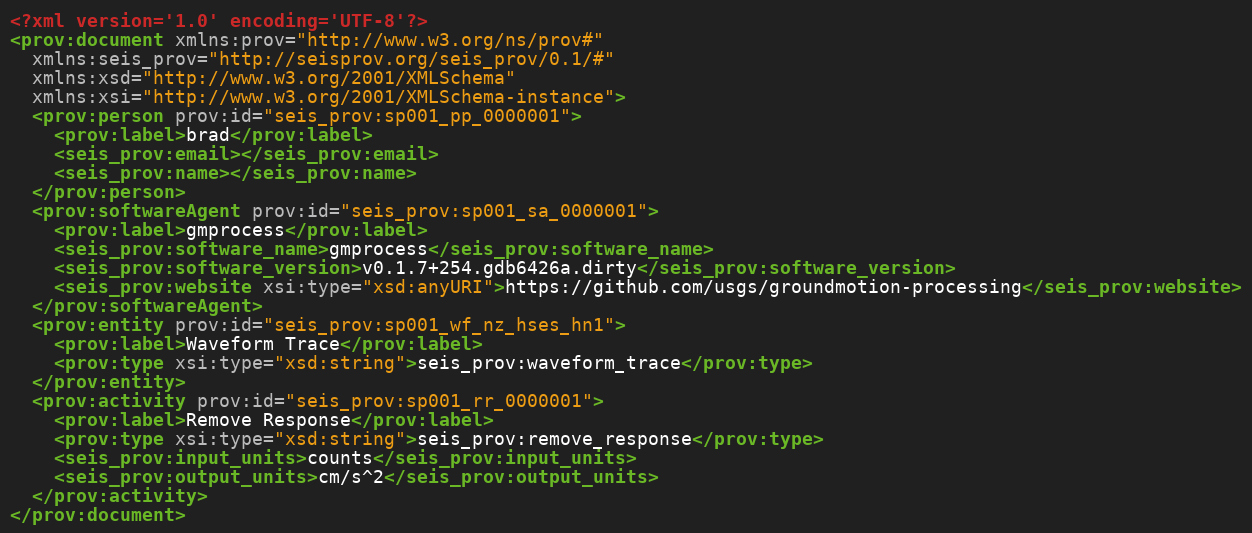
\includegraphics[scale=0.5]{asdf_provxml}};
  
\end{tikzpicture}

\end{document}

